%% Beispiel-Präsentation mit LaTeX Beamer im KIT-Design
%% entsprechend den Gestaltungsrichtlinien vom Februar 2025
%%
%% Siehe https://sdq.kastel.kit.edu/wiki/Dokumentvorlagen

%% Beispiel-Präsentation
\documentclass[
                en,
                % kitgrid
                ]{sdqbeamer} 
 
%% Gruppenlogo, muss im Verezeichnis logos/ liegen
%% falls kein Gruppenlogo gewünscht, bitte \grouplogo{} aufrufen
\grouplogo{} 

%% Gruppenname und Breite (Standard: 89 mm)
\groupname{Institute for Physical Chemistry}
%\groupnamewidth{89mm}

% Beginn der Präsentation

\title[Ex. 2: Regression]{Maschinelles Lernen für die Chemie - Exercise 2}
\subtitle{Bayes' Theorem, Data Types and Regression}
\author[L. Pfeffer, M. Vogelbacher]{Leonie Pfeffer, Maike Vogelbacher}

\date[\today]{\today}

% Literatur 
 
\usepackage[citestyle=numeric,bibstyle=numeric,hyperref,backend=biber]{biblatex}
\addbibresource{presentation.bib}
\bibhang1em

\usepackage{lipsum}
\usepackage{ulem}
\usepackage{amsmath}
\usepackage{tikz}
\usetikzlibrary{trees}

\begin{document}

%Titelseite
\begin{frame}[title blue vertical, picture=images/title_img.png]
% \begin{frame}[title blue vertical, picture=images/palladio_bauplan]
	\titlepage
\end{frame}

\section{Bayes' Theorem}

\begin{frame}{Probabilities and Notation}
    \begin{columns}
        \begin{column}{0.5\textwidth}
            \begin{itemize}
                \setlength\itemsep{2em}
                \item $P(A)$: Probability of observing event $A$
                \item $P(B)$: Probability of observing event $B$
                \item $P(A|B)$: \textbf{Conditional} probability, the probability of
                    event $A$ occurring given that $B$ is true
            \end{itemize}
    \end{column}
    \begin{column}{0.5\textwidth}
        \centering{}
        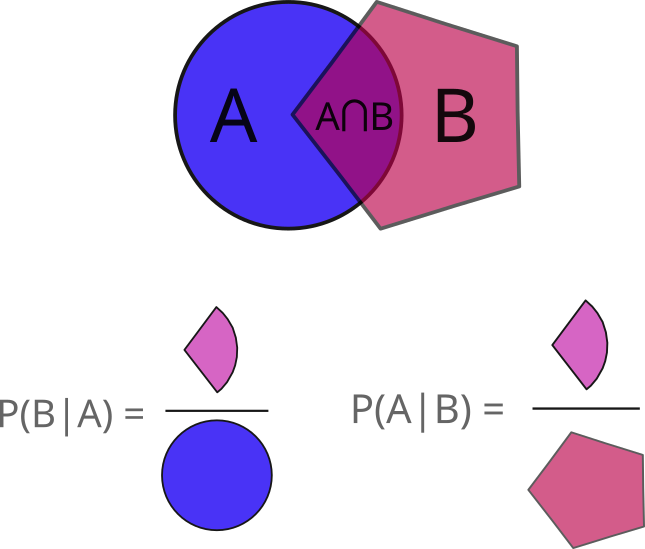
\includegraphics[width=0.8\textwidth]{images/probs.png}
    \end{column}
    \end{columns}
\end{frame}

\begin{frame}{Bayes' Theorem}
    \begin{columns}
        \column{\kitthreecolumns}
        \begin{greenblock}{Mathematical rule for \textbf{inverting conditional
            probabilities}}
            \begin{equation*}
                P(A|B) = \frac{P(B|A) \cdot P(A)}{P(B)}
            \end{equation*}
        \end{greenblock}
        \column{\kitthreecolumns}
            \textbf{Proof:}
            \vfill
            \centering{}
            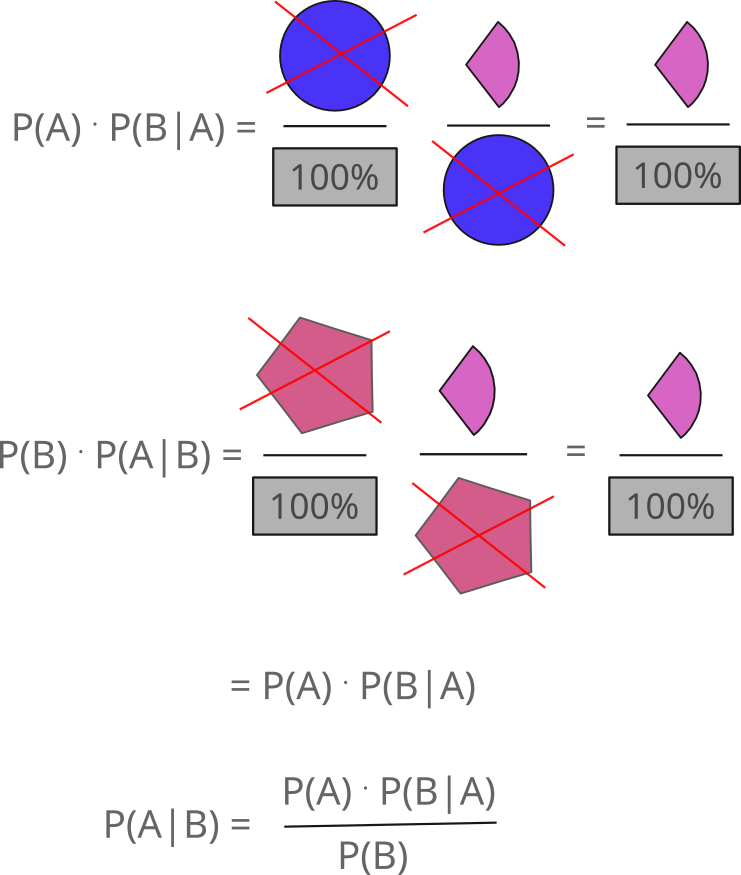
\includegraphics[width=0.7\textwidth]{images/bayes_proof.png}
    \end{columns}
\end{frame}

\begin{frame}{Bayes' Theorem -- Example}
    Testing for an infection ($T$: test positive, $K$ infected people,
    $G$ healthy people)
    \vfill
    \begin{itemize}
        \setlength\itemsep{2em}
        \item Prevalence (people who get infected): $P(K) = 0.0002$
        \item Sensitivity (positive test if person is infected): $P(T|K) = 0.95$
        \item Specificity (positive test if person is healthy): $P(T|G) = 0.01$
        \item Amount of tested people: 100\,000
        \item What is the probability that a random positively tested person is
            actually infected?
        % \item Solution:

        %     \begin{equation*}
        %         P(K|T) = \frac{P(T|K) \cdot P(K)}{P(T)} = \frac{0.95 \cdot
        %         0.0002}{0.95 \cdot 0.0002 + 0.01 \cdot 0.9998} \approx 0.0186
        %     \end{equation*}

        %     with the probability for the positively tested people

        %     \begin{equation*}
        %         P(T) = P(T|K) \cdot P(K) + P(T|G) \cdot P(G)
        %     \end{equation*}
    \end{itemize}
\end{frame}

\begin{frame}{Bayes' Theorem -- Example}
    Testing for an infection ($T$: test positive, $K$ infected people,
    $G$ healthy people)
    \vfill
    \begin{columns}
        \column{\kittwocolumns}
            Prevalence $P(K) = 0.0002$
        \column{\kittwocolumns}
            Sensitivity $P(T|K) = 0.95$
        \column{\kittwocolumns}
            Specificity $P(T|G) = 0.01$
    \end{columns}
    \vfill
    \begin{columns}
        \column{\kittwocolumns}
    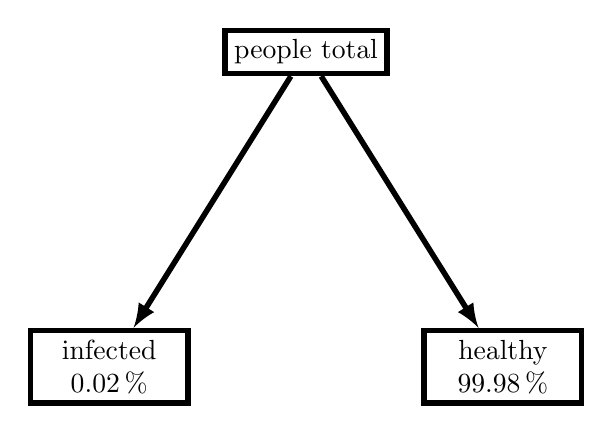
\begin{tikzpicture}[
  level 1/.style={sibling distance=50mm},
  level distance=40mm,
  edge from parent/.style={draw,-latex, line width=2pt},
  every node/.style={draw, rectangle, minimum width=2cm, align=center, line
  width=2pt}
]
\node {people total}
    child {node {infected \\ 0.02\,\%}}
    child {node {healthy \\ 99.98\,\%}};

\end{tikzpicture}
    
        \column{\kittwocolumns}
    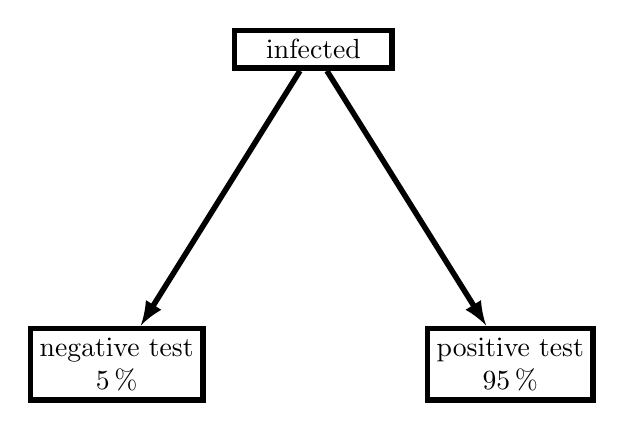
\begin{tikzpicture}[
  level 1/.style={sibling distance=50mm},
  level distance=40mm,
  edge from parent/.style={draw,-latex, line width=2pt},
  every node/.style={draw, rectangle, minimum width=2cm, align=center, line
  width=2pt}
]
\node {infected}
    child {node {negative test \\ 5\,\%}}
    child {node {positive test \\ 95\,\%}};

\end{tikzpicture}

    \column{\kittwocolumns}
    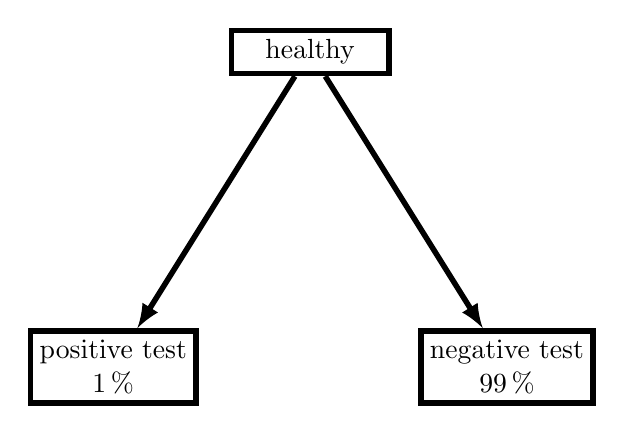
\begin{tikzpicture}[
  level 1/.style={sibling distance=50mm},
  level distance=40mm,
  edge from parent/.style={draw,-latex, line width=2pt},
  every node/.style={draw, rectangle, minimum width=2cm, align=center, line
  width=2pt}
]
\node {healthy}
    child {node {positive test \\ 1\,\%}}
    child {node {negative test \\ 99\,\%}};

\end{tikzpicture}
    \end{columns}
\end{frame}

\begin{frame}{Bayes' Theorem -- Example}
    \begin{columns}
        \begin{column}{0.7\textwidth}
    \centering
    \begin{tikzpicture}[
  level 1/.style={sibling distance=100mm},
  level 2/.style={sibling distance=50mm},
  level distance=40mm,
  edge from parent/.style={draw,-latex, line width=2pt},
  every node/.style={draw, rectangle, minimum width=2cm, align=center, line
  width=2pt}
]
\node {people total \\ 100\,000}
    child {node {infected \\ 20}
    child {node {negative test \\ 1}}
    child {node [fill=kit-green50] {positive test \\ 19}}
  }
  child {node {healthy \\ 99\,980}
    child {node [fill=kit-green50] {positive test \\ 1000}}
    child {node {negative test \\ 98\,980}}
  };
\end{tikzpicture}
\end{column}
\begin{column}{0.3\textwidth}
    \begin{equation*}
        P(K|T) = \frac{P(T|K) \cdot P(K)}{P(T)}
    \end{equation*}
\end{column}
\end{columns}

\end{frame}

\begin{frame}{Bayes' Theorem -- Example}
    \textbf{Solution:}
    \vfill 
    \begin{equation*}
        P(K|T) = \frac{P(T|K) \cdot P(K)}{P(T)} = \frac{0.95 \cdot
        0.0002}{0.95 \cdot 0.0002 + 0.01 \cdot 0.9998} \approx 0.0186
    \end{equation*}
    \vfill 
    with the probability for the positively tested people
    \vfill 
    \begin{equation*}
        P(T) = P(T|K) \cdot P(K) + P(T|G) \cdot P(G)
    \end{equation*}
\end{frame}

\section{Data Types}

\begin{frame}{What Are Data Types?}
    \begin{itemize}
        \setlength\itemsep{2em}
        \item Each variable has a data type
        \item Other programs: data type has to be set by the user \\
            Python: \textbf{dynamic typing}, data type is declared automatically
        \item Data type is important, because it determines:
    \end{itemize}

    \vfill

    \begin{enumerate}
        \setlength\itemsep{1em}
        \item the amount of memory used for this variable
        \item the attributes of the variable (i. e. elements of a list
            can be accessed, accessing the elements of an integer
            doesn't make sense)
    \end{enumerate}
    
\end{frame}

\begin{frame}{Examples for Data Types in Python}

    \begin{itemize}
        \setlength\itemsep{2em}
        \item Integer: \texttt{x = 2}
        \item Floats: \texttt{pi = 3.1415}
        \item String: \texttt{"Some random text"}
        \item List: \texttt{my\_list = [1, 2, 3]}
        \item Dictionary: \texttt{my\_dict = \{key: value\}}
        \item Boolean: \texttt{condition = True}
    \end{itemize}

\end{frame}

\begin{frame}{Type Hints}
    \begin{itemize}
        \setlength\itemsep{2em}
        \item Example: \texttt{x: int = 2}
        \item States directly, that \texttt{x} should be an integer
        \item In the notebooks: used for hints what to do
    \end{itemize}
    \vfill
    \centering
    \colorbox{kit-gray30}{\parbox{0.8\textwidth}{
            \texttt{x: int}

            \texttt{y: np.ndarray}

            \texttt{\# Your code:}

            \texttt{x = 100  \# Sample size}

            \texttt{y = np.arange(100)  \# Numpy array with all values from 0 to
            99}
    }}
    
\end{frame}

\section{Regression}

\begin{frame}{Linear Regression}
    \begin{columns}
        \column{\kitthreecolumns}
            \begin{itemize}
                \item Input vector (features) $X$
                \item Response (label, target) $Y$
            \end{itemize}
            \centering
            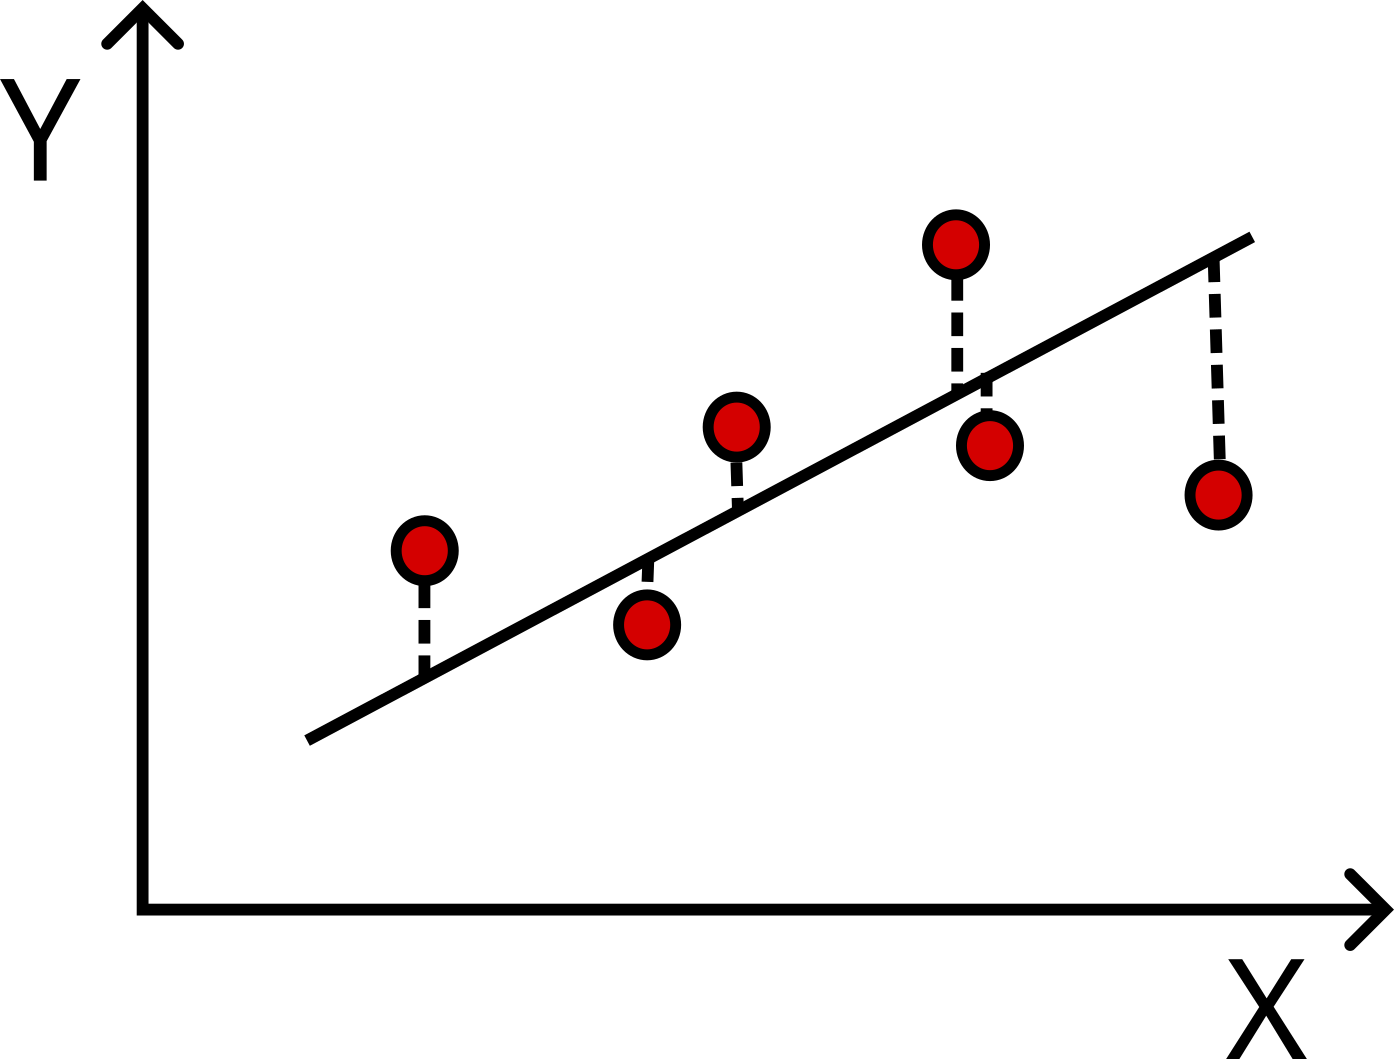
\includegraphics[width=0.8\textwidth]{images/lin_reg.png}

        \column{\kitthreecolumns}
            \begin{equation}
                f(X) = \beta_0 + \sum_{j} X_j \beta_j
            \end{equation}

            With the set of training data $(x_i, y_i)$, we minimize the
            \textbf{residual sum of squares}:

            \begin{align}
                \text{RSS}(\beta) &= \sum_i (y_i - f(x_i))^2 \\
                                  &= \sum_i \left(y_i - \beta_0 - \sum_j x_{ij}
                                  \beta_j \right)^2
            \end{align}
    \end{columns}
\end{frame}

\begin{frame}{Linear Regression -- Matrix Notation}
    \begin{itemize}
        \setlength\itemsep{2em}
        \item Write the input vectors of the features $X_j$ as a matrix
            $\boldsymbol{X}$ of shape $N \times p$ ($N$: number, $p$ length of
            input vectors)
        \item Include intersect (bias) $\beta_0$ in the feature matrix
            $\boldsymbol{X}$ as a column of ones $\Rightarrow$ new shape: $N
            \times (p+1)$
        \item $y$: $N$-vector of outputs in the training set
        \item RSS can be expressed as:

            \begin{equation*}
                \text{RSS}(\beta) = (\boldsymbol{y} - \boldsymbol{X} \beta)^T
                (\boldsymbol{y} - \boldsymbol{X} \beta)
            \end{equation*}
    \end{itemize}
\end{frame}

\begin{frame}{Linear Regression -- Parameters}
    \begin{columns}
        \column{\kitthreecolumns}
        \begin{greenblock}{Minimizing the RSS in the matrix form leads to a
            unique solution for the parameters:}
                \begin{equation*}
                    \hat{\beta} = (\boldsymbol{X}^{T} \boldsymbol{X})^{-1}
                    \boldsymbol{X}^T \boldsymbol{y}
                \end{equation*}
    \end{greenblock}
        \begin{itemize}
            \setlength\itemsep{2em}
            \item $\boldsymbol{X}$: $N \times (p+1)$ matrix, $N$ input vectors
                as rows, $p$ length of input vectors, $1$ in the first position
                (to account for $\beta_0$) \item $\boldsymbol{y}$: $N$-vector of
                outputs in the training set
        \end{itemize}

        \column{\kitthreecolumns}
        Exercise:
        \begin{itemize}
            \setlength\itemsep{2em}
            \item Features $\boldsymbol{X}$: medical information
                ($N_\text{test} \times 11$, first column consisting of ones)
            \item Target $\boldsymbol{y}$: diabetes or not ($N_\text{test}$)
        \end{itemize}
    \end{columns}
\end{frame}

\begin{frame}{Linear Regression -- Exercise}
    \begin{itemize}
        \setlength\itemsep{2em}
        \item Split the data in two random subsets for training and testing \\
            $\Rightarrow$ Scikit-learn:
            \texttt{train\_test\_split(feature\_array, target\_array,
            test\_size=?, random\_state=0)}
        \item Insert column of ones to the training set $\boldsymbol{X}$ \\
            $\Rightarrow$ Numpy array of ones:
            \texttt{np.ones((train\_set.shape[0], 1))} \\
            $\Rightarrow$ Prepend the array to the training set:
            \texttt{np.concatenate((ones\_array, train\_set), axis=1)}
        \item Calculate $\hat{\beta}$ with the prepended training matrix and the
            targets: \\
            Matrix multiplication: $\Rightarrow$ Numpy \texttt{np.matmul} or \texttt{@} \\
        Invert matrix: $\Rightarrow$ \texttt{np.linalg.inv} \\
        Transpose matrix: $\Rightarrow$ \texttt{matrix.T}
    \end{itemize}
\end{frame}

\begin{frame}{Linear Regression -- Exercise}
    Or completely with Scikit-learn:

    \vfill

    \begin{itemize}
        \setlength\itemsep{2em}
        \item Create a linear regression instance:  \\
            $\Rightarrow$ \texttt{model: LinearRegression = LinearRegression()}
        \item Train your model: \\
            $\Rightarrow{}$ \texttt{model.fit(train\_set, target\_set)}
        \item Test the model by predicting the targets with the test set: \\
            $\Rightarrow{}$ \texttt{model.predict(test\_set)}
        \item Save the parameters $\hat{\beta}$ as one Numpy array by inserting
            the interception at position $0$ to the other coefficients: \\
            $\Rightarrow{}$ \texttt{np.insert(model.coef\_, 0, model.intercept\_,
            axis=0)}
    \end{itemize}
    
\end{frame}

\begin{frame}{Today's Notebooks}
    \texttt{2.1\_Numpy\_Crashcourse.ipynb}
    \begin{itemize}
        \item Optional, from Ex. 1
    \end{itemize}
    \vfill
    \texttt{1.1\_LogisticRegressionTutorial.ipynb}
    \begin{itemize}
        \item Logistic regression tutorial to predict the subspecies of an iris flower
        \item Look here, if you need hints for the exercise notebook
    \end{itemize}
    \vfill
    \texttt{1.2\_RegressionExercise.ipynb}
    \begin{itemize}
        \item Linear regression exercise as explained earlier
        \item Quantification of the results: refer to tutorial
        \item Polynomic regression: similar to linear regression, use
            appropriate Scikit-learn object
        \item Lasso regression as regularization example, again, different
            Scikit-learn object but otherwise similar
    \end{itemize}
\end{frame}

\appendix
% Slides form here will not be counted in the page numbering nor will they
% appear in the navigation bar
\beginbackup

\begin{frame}{Literature}
    \begin{itemize}
        \setlength\itemsep{2em}
        \item Linear Regression~\nocite{Hastie-2009}
            \printbibliography[keyword={hastie},title={Linear Regression}]
        \item Bayes' theorem and probabilities~\nocite{wikipedia-bayes-en,
            wikipedia-bayes-de}
            \printbibliography[keyword={bayes}, title={Bayes' theorem and
            probabilities}]
    \end{itemize}
\end{frame}

\backupend
\end{document}
